\chapter{Détection de groupes pertinents dans les flots de liens}
\minitoc
Nous avons vu précédemment qu'il était possible de trouver des groupes de liens dans un flots de liens via l'intermédiaire d'une projection du flot de liens en un graphe statique.
Parmi l'ensemble de ces groupes, il se peut que certains capturent des structures plus importantes et plus pertinentes que d'autres.
Le but ici est de réussir à extraire parmi ces groupes ceux qui sont pertinents.
En ce sens, nous nous posons la question de la décomposition partielle d'un flot de liens en sous-flots pertinents.
Il s'agit donc d'un problème légèrement différent de la détection de partition car certains liens peuvent n'appartenir à aucun groupe et les groupes doivent être pertinents.

Toute la difficulté pour réussir à trouver les groupes pertinents revient à trouver une définition convaincante de la pertinence.
La notion de densité est une première approche mais ce n'est pas suffisant.
En effet comme on a pu le voir précédemment, il peut exister de très grand groupes peu dense et de petits groupes très denses.
Faire la différence entre ces deux catégories en utilisant juste la densité n'est pas possible.
C'est pourquoi, nous utilisons une notion de voisinage.
Un groupe est alors pertinent si il est plus dense que son voisinage.
Ainsi, un groupe peu dense peut être pertinent si il est plus dense que son voisinage.
Comme le but est de pouvoir décrire le flot de liens, nous nous limitons aux groupes ayant une taille supérieur à un minimum.
Un exemple de flots avec une décomposition en groupes pertinent est dans la figure~\ref{fig:exemple_groupe_dens}.

Afin de trouver des des groupes pertinents, nous procédons de la manière suivantes:
\begin{itemize}
\item Nous construisons la projection du flot de liens en un graphe statique;
\item Nous appliquons sur cette projection un algorithme de détection de communautés afin d'obtenir une partition des liens du flot de liens;
\item Nous ne gardons dans la partition que les groupes qui sont considérés comme pertinent, c'est-à-dire ceux qui sont assez gros et qui sont plus dense que leur voisinage.
\end{itemize}

Afin de montrer la pertinence de cette approche, nous l'appliquons sur différents jeux de données et essayons de faire une analyse manuelle de certains groupes trouvés.
Par ailleurs, nous montrons que les groupes que nous détectons ne le sont pas par une méthode statique.

Le chapitre est organisé de la manière suivante.
Dans la section~\ref{sec:groupe_dense_existant}, nous revenons sur les travaux existants qui traitent de sujets similaire.
Puis dans la section~\ref{sec:groupe_dense_method}, nous présentons notre méthode de détection et de validation de groupes pertinents.
Enfin, les jeux de données que nous utilisons sont présentés dans la section~\ref{sec:groupe_dense_result} et les résultats associés dans la section~\ref{sec:groupe_dense_data}.

\begin{figure}
\centering
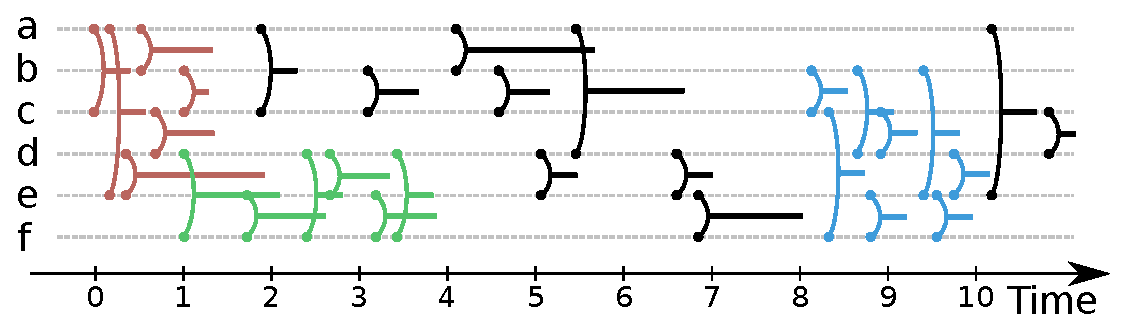
\includegraphics[width=\linewidth]{img/GroupeDense/GroupExample/Zone_dense.eps}
\caption{Exemple de flots de liens avec 3 groupes denses représenté par la couleur des liens (\textcolor{brique}{\textbf{rouge}}, \textcolor{vert_turquoise}{\textbf{vert}} et \textcolor{bleu_window}{\textbf{bleu}}).
}
\label{fig:exemple_groupe_dens}
\end{figure}

\section{Travaux existants}
\label{sec:groupe_dense_existant}

Comme nous l'avons vu dans le chapitre~\ref{chap:etat_art}, il existe assez peu de méthodes cherchant une structure dans un formalisme sans perte d'information.

Mitra~\emph{et al.}~\cite{Mitra2012a} et Speidel~\emph{et al.}~\cite{Speidel2015} ont développé une méthode de détection de communauté mais dans les réseaux diachronique.
Dans un tel réseau, ce sont les n\oe uds qui ont un \emph{timestamp} et non les liens.
Ce cas de figure s'applique parfaitement aux citations car une citation relie bien deux publications qui sont chacune apparues à une date spécifique.
Cependant ce genre de construction est différente n'est pas équivalente au formalisme de flot de liens.
C'est pourquoi nous ne pouvons utiliser la même méthode. 

Ils existent également des méthodes capturant la partie la plus dense du réseau.
C'est le cas de Bogdanov~\emph{et al.}~\cite{Bogdanov2011} qui considèrent encore une autre variante d'extension de graphe.
Ils considèrent un graphe dont la topologie n'évolue pas mais dont le poid des liens change en fonction du temps entre $-1$ et $1$.
Ce formalisme est encore une fois très différent de celui de flot de liens.
De plus, la notion de densité qu'ils utilisent ne tiens pas vraiment compte du temps.
En effet, un groupe de n\oe uds sur intervalle est évalué par la somme des liens entre ces n\oe uds sur tout l'intervalle.


Epasto~\emph{et. al}~\cite{Epasto2015} capture le sous-graphe le plus dense dans un graphe temporel.
Ainsi, le temps est bien pris en compte dans le formalisme.
Cependant, la méthode capture le sous-graphe à un instant $t$ qui est le plus dense.
La notion de densité est donc statique car elle ne considère que la structure de graphe à l'instant $t$.


Enfin il existe les travaux de Rozenshtein~\emph{et. al}~\cite{rozenshtein2014} qui se rapprochent le plus de notre méthode.
Leur méthode considère le formalise de flots de liens et ne suppose pas de structure de graphe à un instant donné.
Elle capture un groupe de n\oe uds et plusieurs intervalles disjoints de telle sorte que ce groupe de n\oe uds dans le graphe agrégé sur ces intervalles ait le degré moyen le plus élevé.
Ainsi même si la méthode permet de capturer un groupe de n\oe uds sur des intervalles, elle évalue un candidat sur le graphe agrégé pour appliquer une métrique de graphe.
Le temps n'a donc pas d'influence sur l'évaluation.
Par ailleurs, leur méthode repose sur plusieurs paramètres qui doivent être fixés \emph{a priori}: le nombre maximum d'intervalle disjoint et la duré cumulée maximum de ces intervalles.
Le premier paramètre permet d'éviter d'utiliser une infinité d'intervalle qui seraient chacun centré sur un lien.
Le second paramètre permet d'éviter de considérer tout le graphe agrégé et ainsi d'obliger la prise en compte du temps.
Ainsi, leur méthode dépend de manière non triviale sur le choix des paramètres.

\bigskip

Pour résumer, il existe des méthodes cherchant la structure la plus dense dans un contexte dynamique; soit en considérant un graphe temporel soit en considérant un flot de liens.
Cependant, ces méthodes utilisent des métriques de graphes pour évaluer un groupe de n\oe uds.
Le temps n'est donc complètement pris en compte dans l'évaluation.
De manière plus importante, ces méthodes évaluent de manière absolue sans prendre en compte de notion de voisinage.
Enfin, nous capturons plusieurs groupes de liens alors qu'ils capturent un groupe n\oe ud.
Certaines des méthodes existantes peuvent être étendues pour capturer les $k$ groupes de n\oe uds les plus denses mais cela se fait au prix de l'ajout d'un paramètre pour contrôler le chevauchement entre deux groupes capturés.


\section{\'Evaluation de la pertinence d'un groupe}
\label{sec:groupe_dense_method}

\section{Jeux de données}
\label{sec:groupe_dense_data}
\section{Application}
\label{sec:groupe_dense_result}



\section{Conclusion et perspective}


\subsection{Jeux de test ?}